\section{Verification and analysis}
\label{sec:verification}

In this section, we present the verification of the segmentation method
described in \Cref{sec:method}. First we qualitatively verify that our method
is sound by comparing the segmentation results to the original tomography and
creating an artificial ground truth. Then we quantitatively verify our method
by generating synthetic data, evaluating it on the created ground truth, and
comparing the results to other existing methods. Finally, we analyze the
segmented data to study the blood vessel network in the bone region and produce
statistics on the tissue-to-implant contact.

\subsection{Qualitative verification}

Since the SRµCT tomograms are clear enough that humans can distinguish between
blood vessels and bone, as our mammalian visual cortex automatically corrects
for the distortion effects, we can verify the success of the automatic
classification. We can compare the automatic classification with the manual
classification of the histological microscopy. A larger quantitative study is
planned that analyses the full data set against recently conducted histological
microscopy taken from the same biopsies.

Figures \Cref{fig:histology-comparison1} and \Cref{fig:histology-comparison2}
show the same 2D slices as were shown in Figures \Cref{fig:3viewsample} and
\Cref{fig:slices}, allowing us to visually inspect them side by side. The
voxels are colored according to the segmentation confidence, with the degree of
red being proportional to the modeled probability $\Pof{0}{v,\fval}$ and the
degree of yellow being proportional to $\Pof{1}{v,\fval}$. Grey voxels indicate
low model probabilities of both: either due to the voxel belonging to another
material or simply low computed confidence of the model.  By comparing the
images in \Cref{fig:histology-comparison1} and
\Cref{fig:histology-comparison2}, we see that the global thresholding (bottom
right) fails to capture the soft tissue close to the implant, which further
confirms the need for a more sophisticated method. Looking at the Otsu
segmentation (top right), we see that it better captures the soft tissue close
to the implant, but still fails even closer to the implant. Our method (bottom
left) captures the soft tissue close to the implant, while still ensuring a
good segmenting in previously well segmented regions.

\begin{figure*}
    \centering
    \begin{tabular}{cc}
        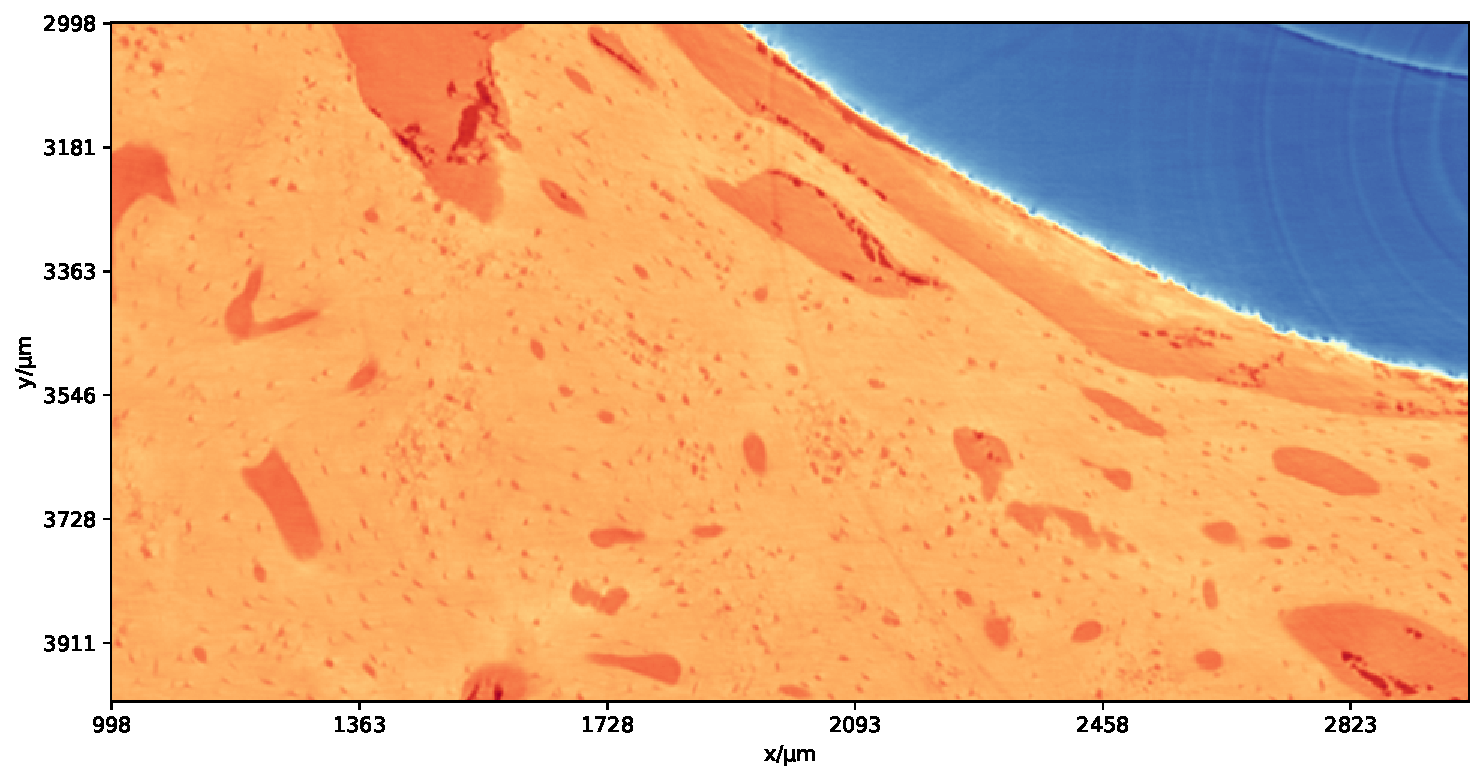
\includegraphics[width=.45\linewidth]{generated/770c_pag_segmented_yx_raw.pdf} &
        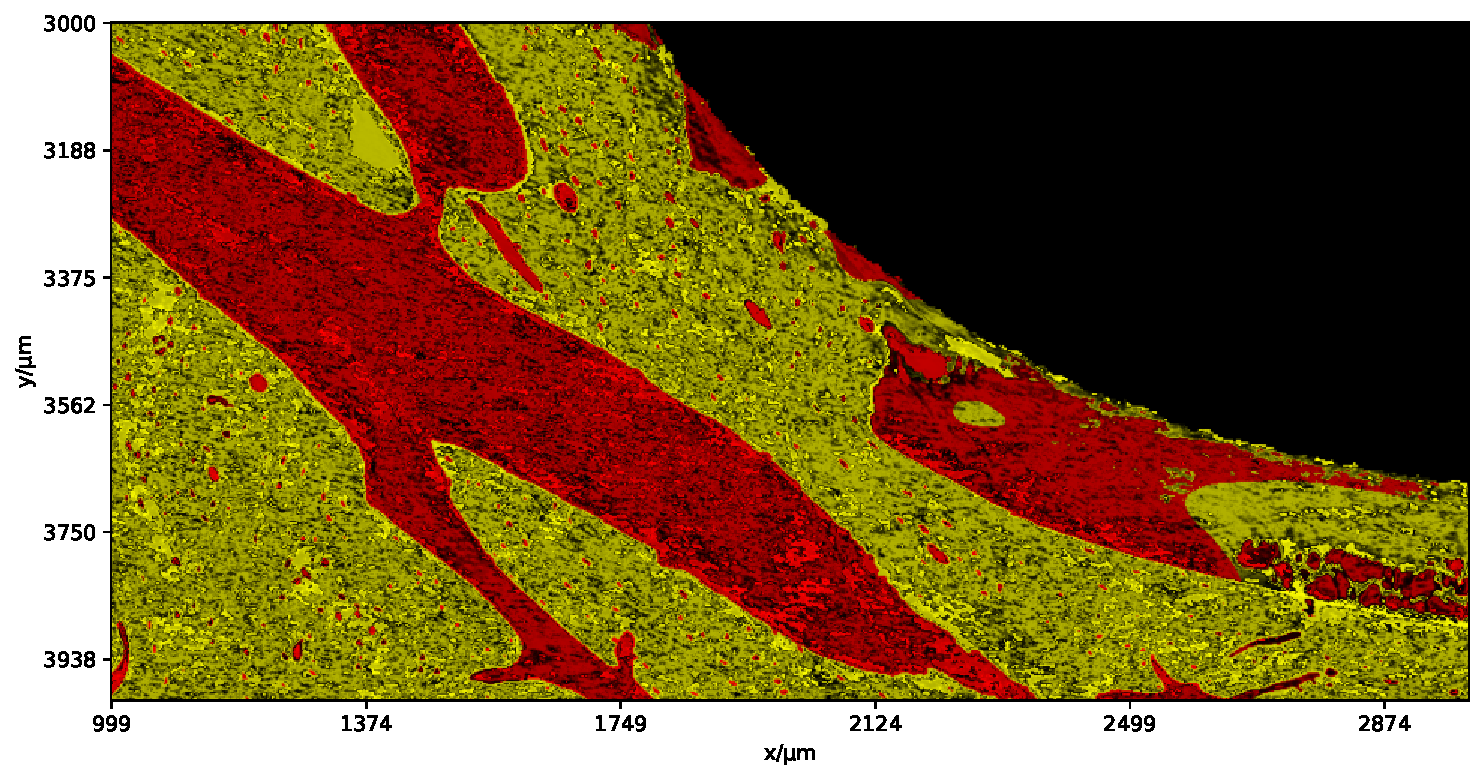
\includegraphics[width=.45\linewidth]{generated/770c_pag_global_yx_otsu.pdf}
        \\
        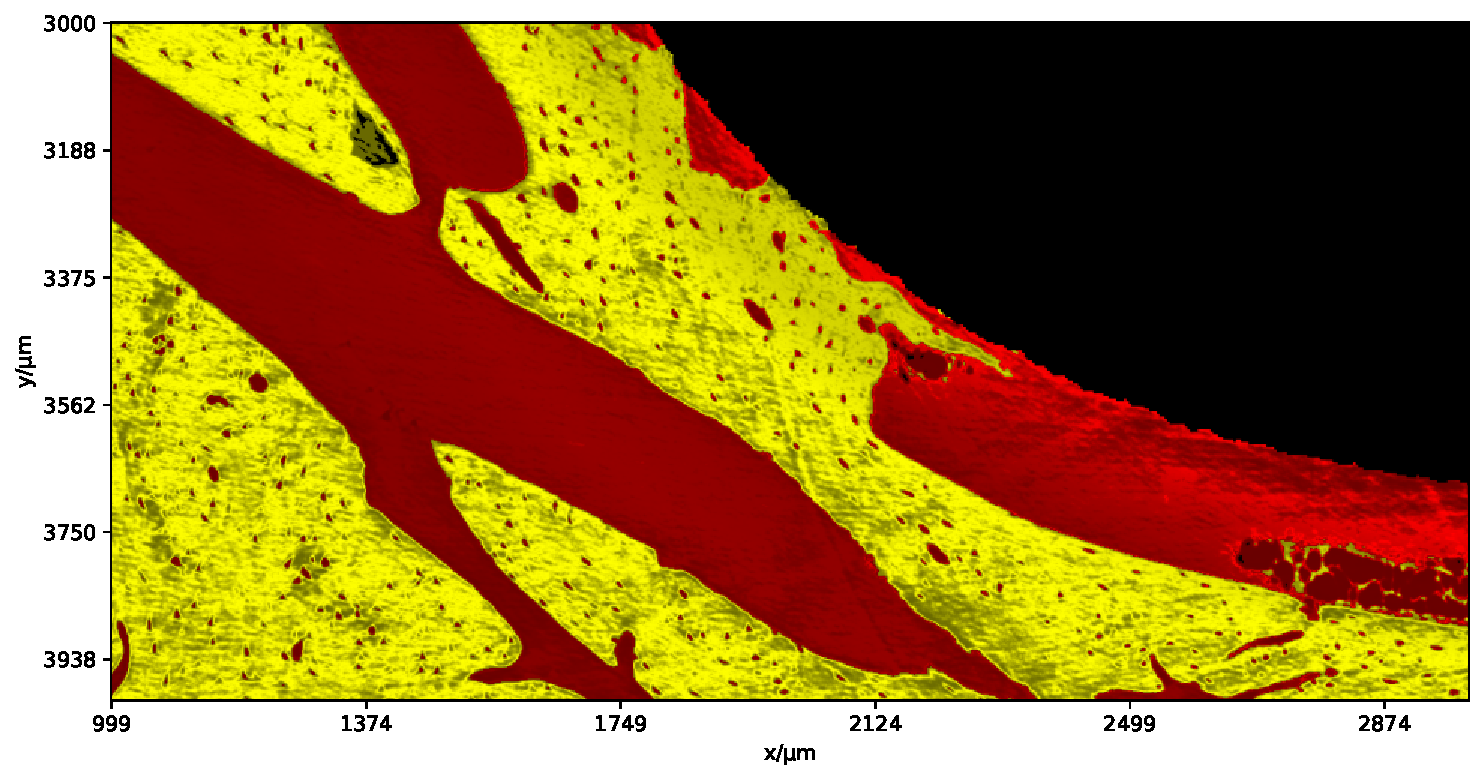
\includegraphics[width=.45\linewidth]{generated/770c_pag_segmented_yx_colored.pdf} &
        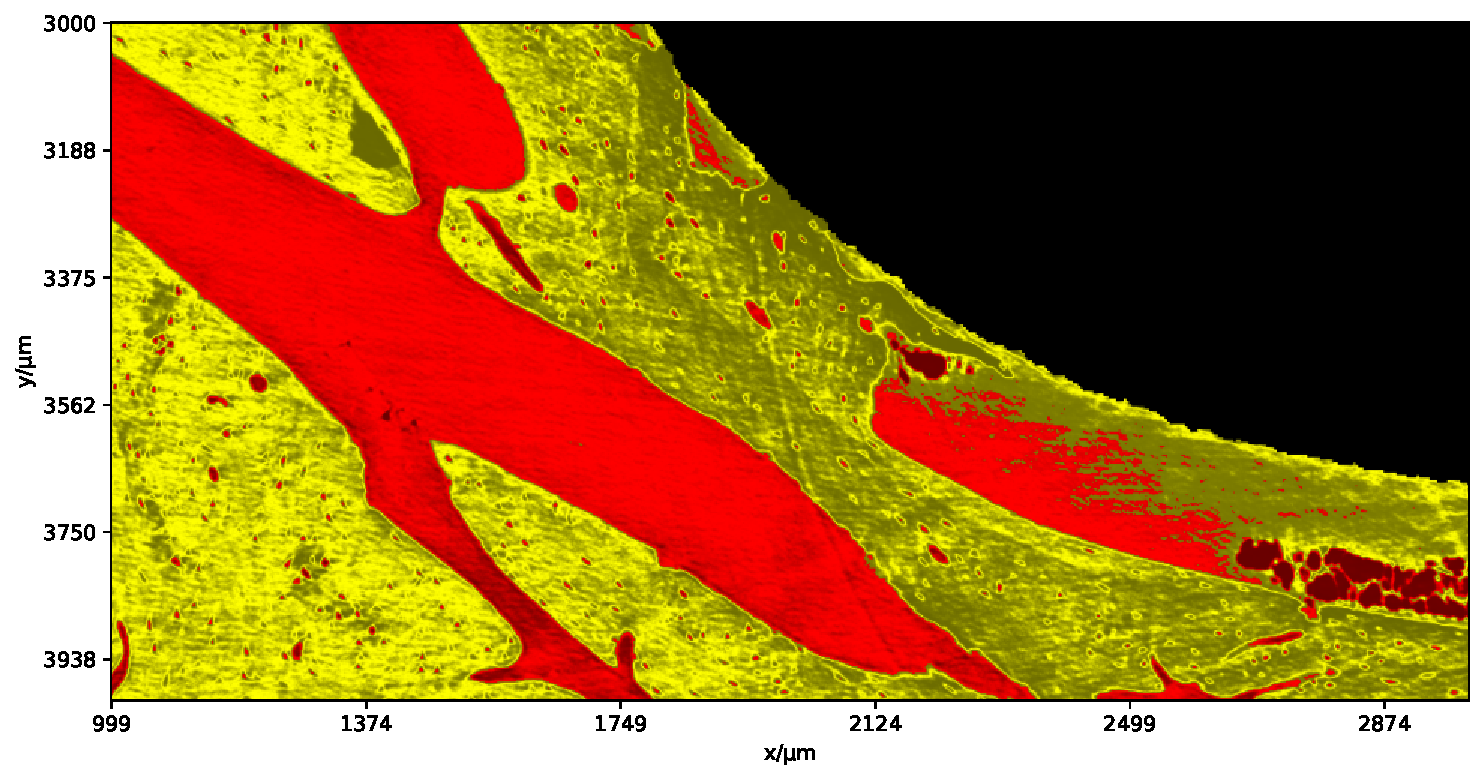
\includegraphics[width=.45\linewidth]{generated/770c_pag_global_yx.pdf} \\
    \end{tabular}
    \caption{
        % TODO (Alle): instead of writing what is what in caption, it would be great to add
	% sub-titles to each figure. Right now it is a bit confusing. Also if would shorten
	% the caption text a bit!
	YX-slices of the original tomography (top left), Otsu segmentation (top
	right), our classification (bottom left), and global threshold
	classification (bottom right).  For our classification, the voxels are
	colored according to the modeled probability functions $P(m\vert
	v,\fval)$ between 0 and 1: completely red voxels have $P(m=0\vert
	v,\fval) = 1$, completely yellow voxels have $P(m=1\vert v,\fval)\ =
	1$, and uncertain voxels become progressively gray.
    }
    \label{fig:histology-comparison1}
\end{figure*}

\begin{figure*}
    \centering
    \begin{tabular}{cc}
        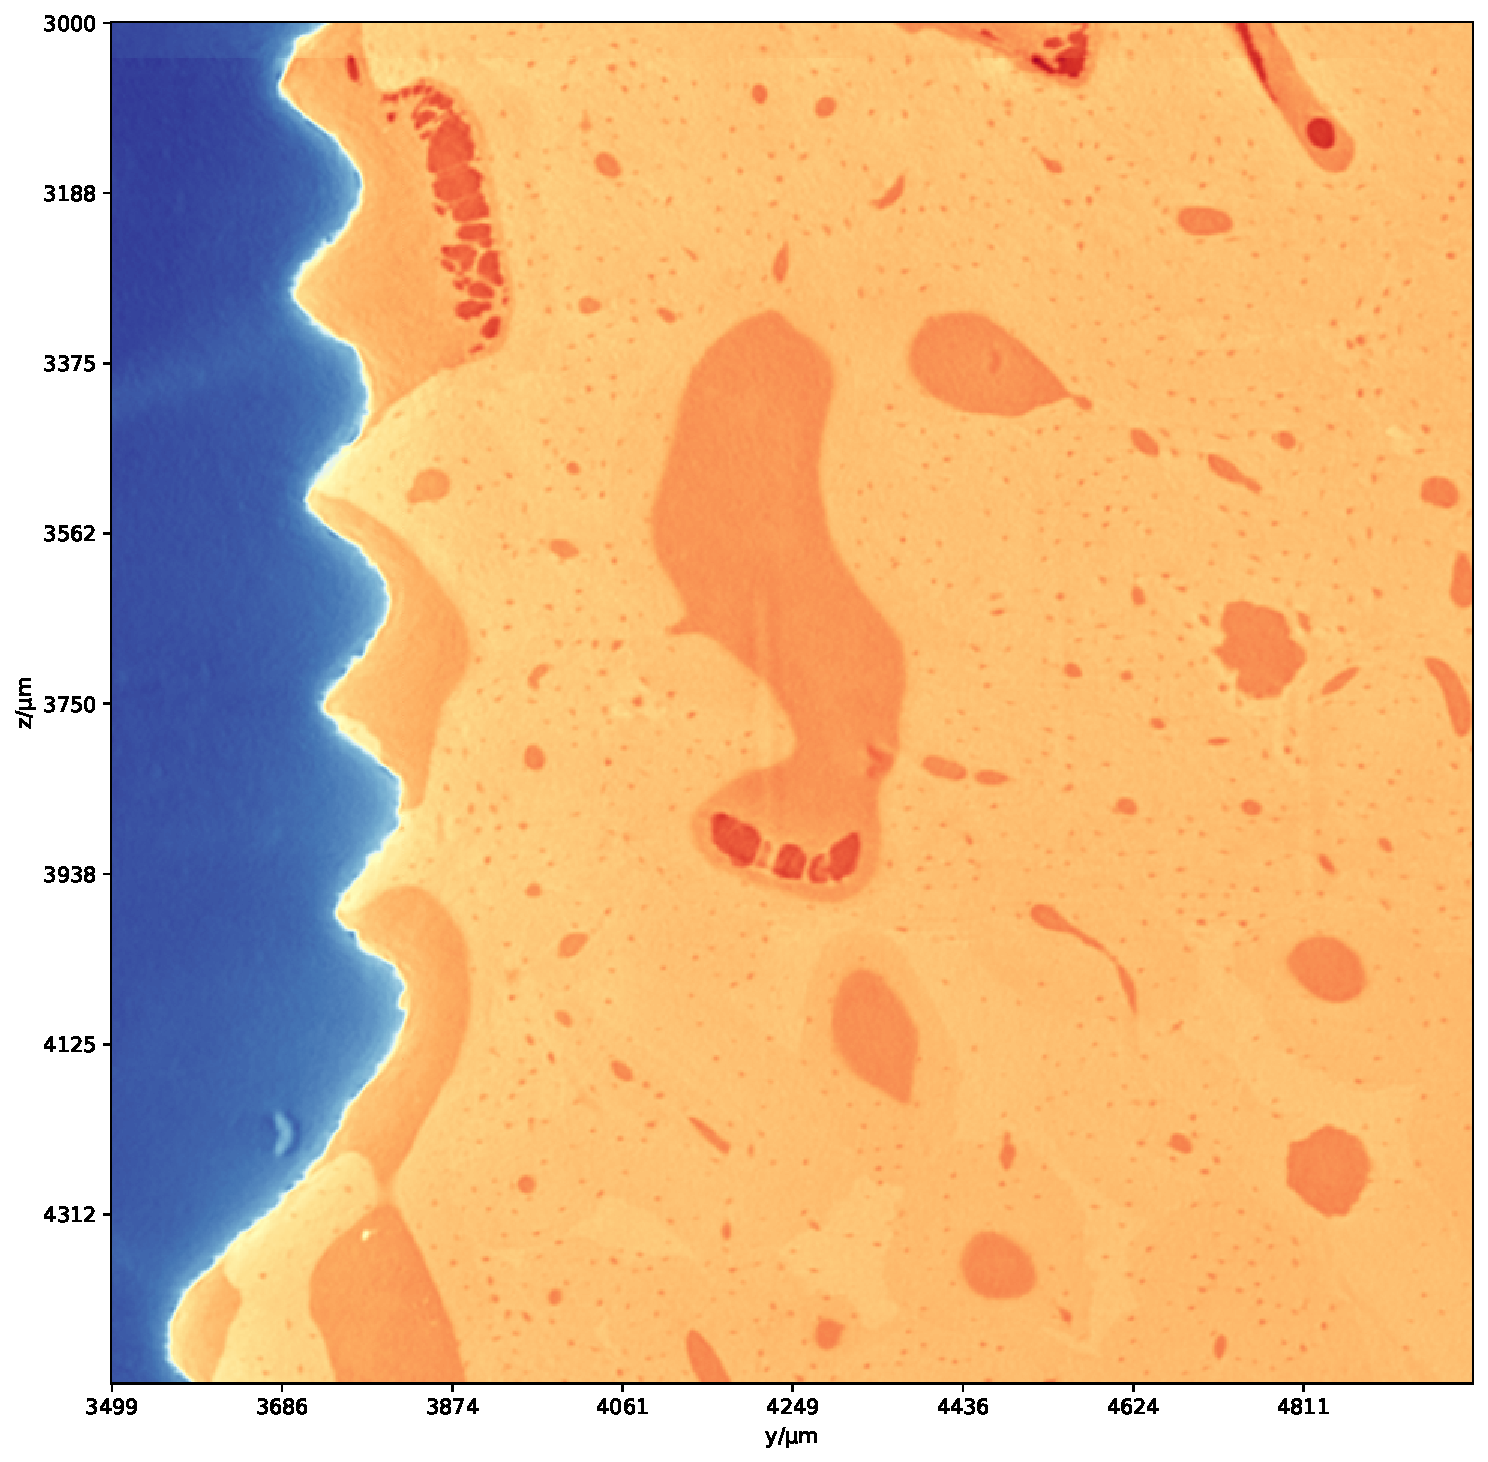
\includegraphics[width=.45\linewidth]{generated/770c_pag_segmented_zy_raw.pdf} &
        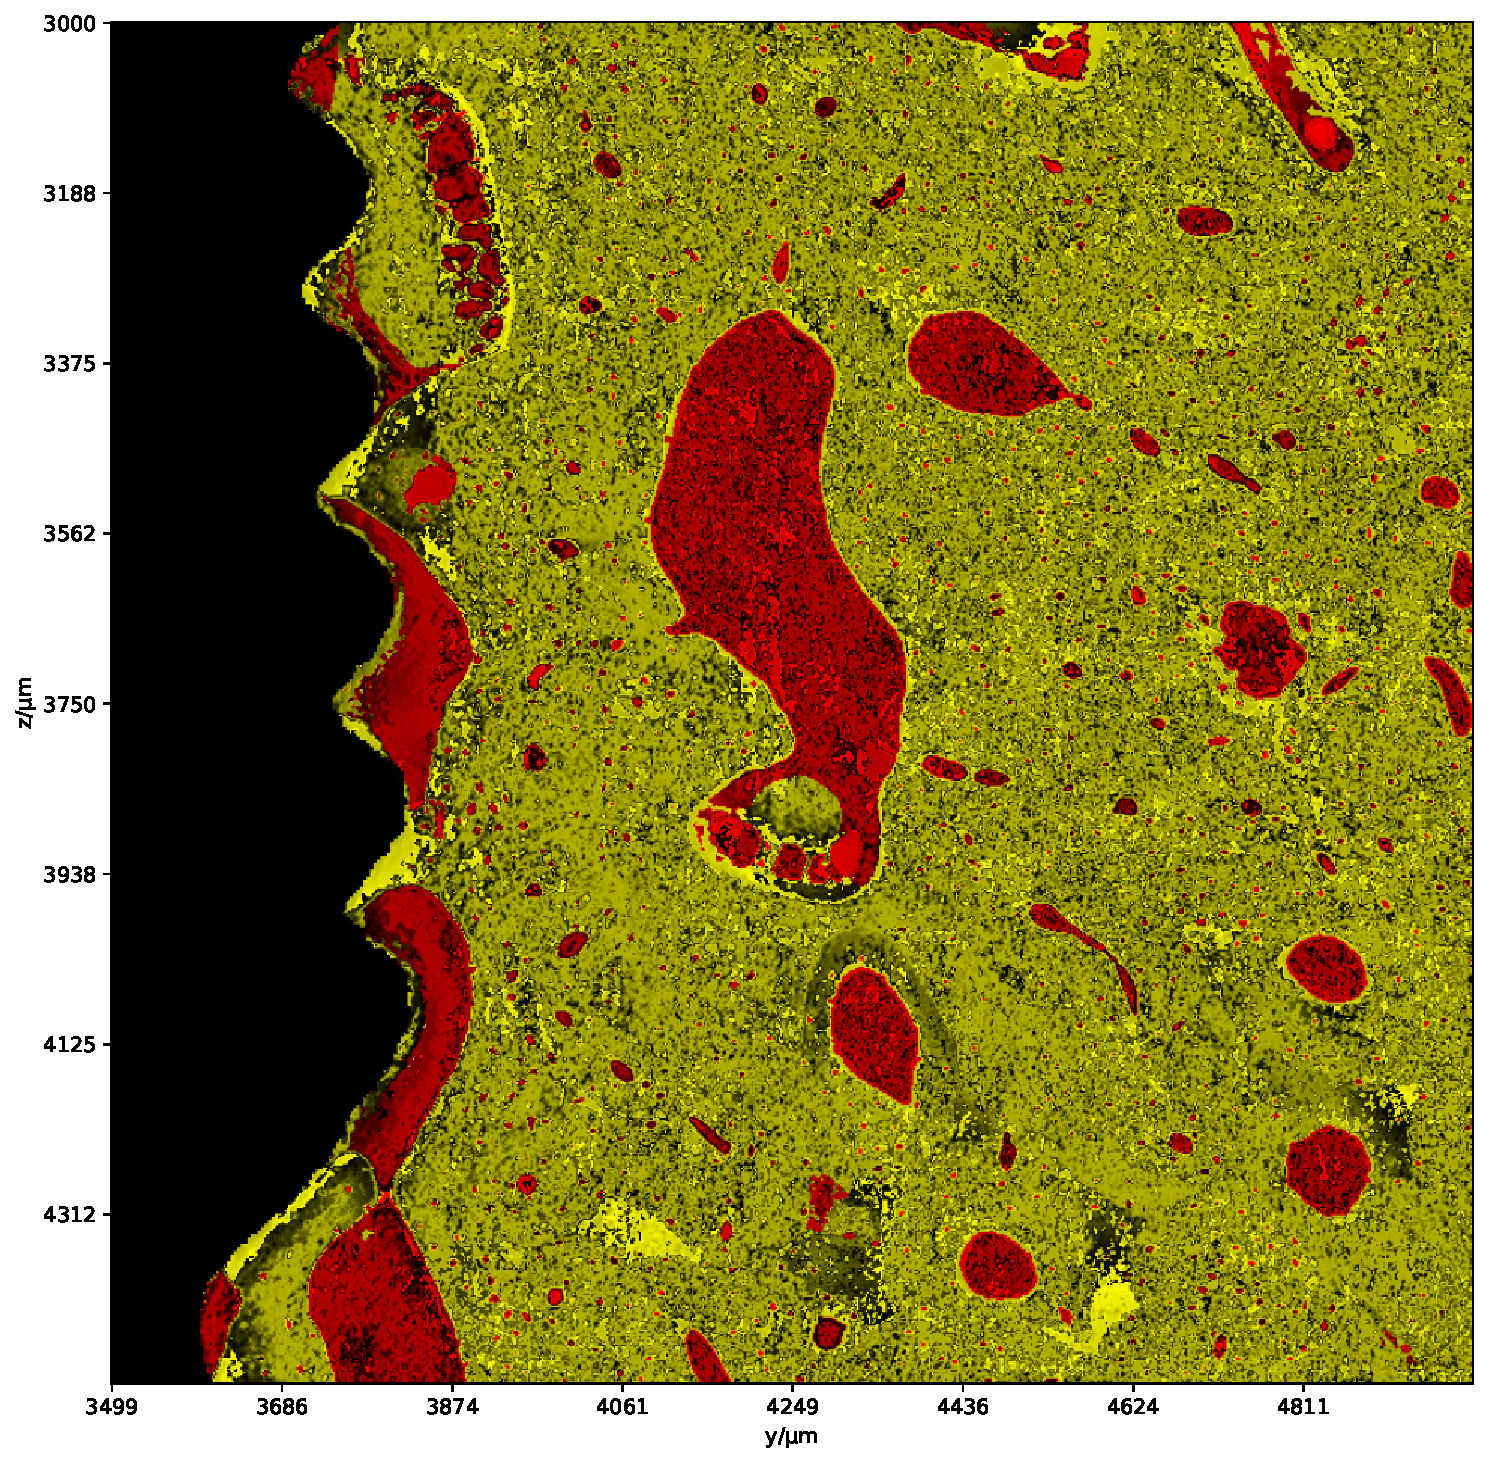
\includegraphics[width=.45\linewidth]{generated/770c_pag_global_zy_otsu.pdf}
        \\
        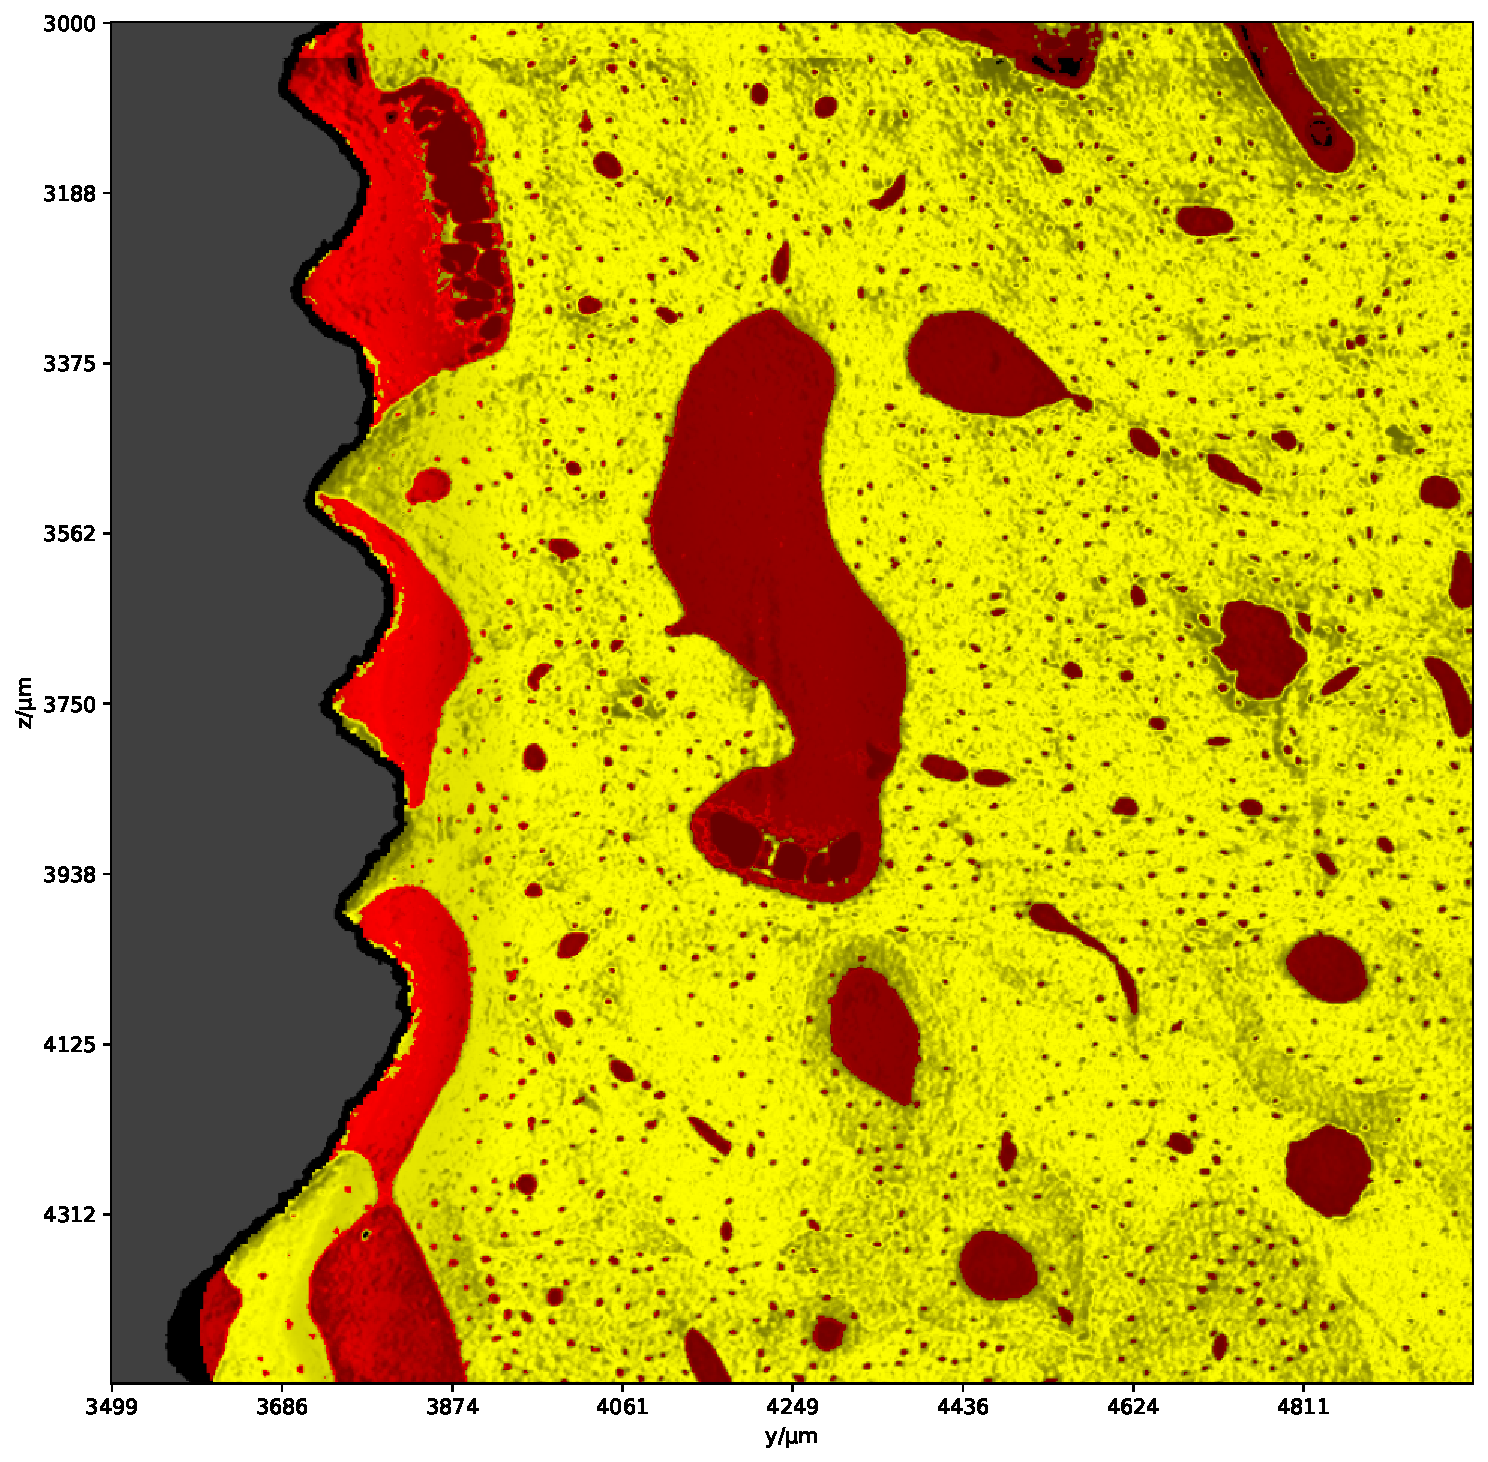
\includegraphics[width=.45\linewidth]{generated/770c_pag_segmented_zy_colored.pdf} &
        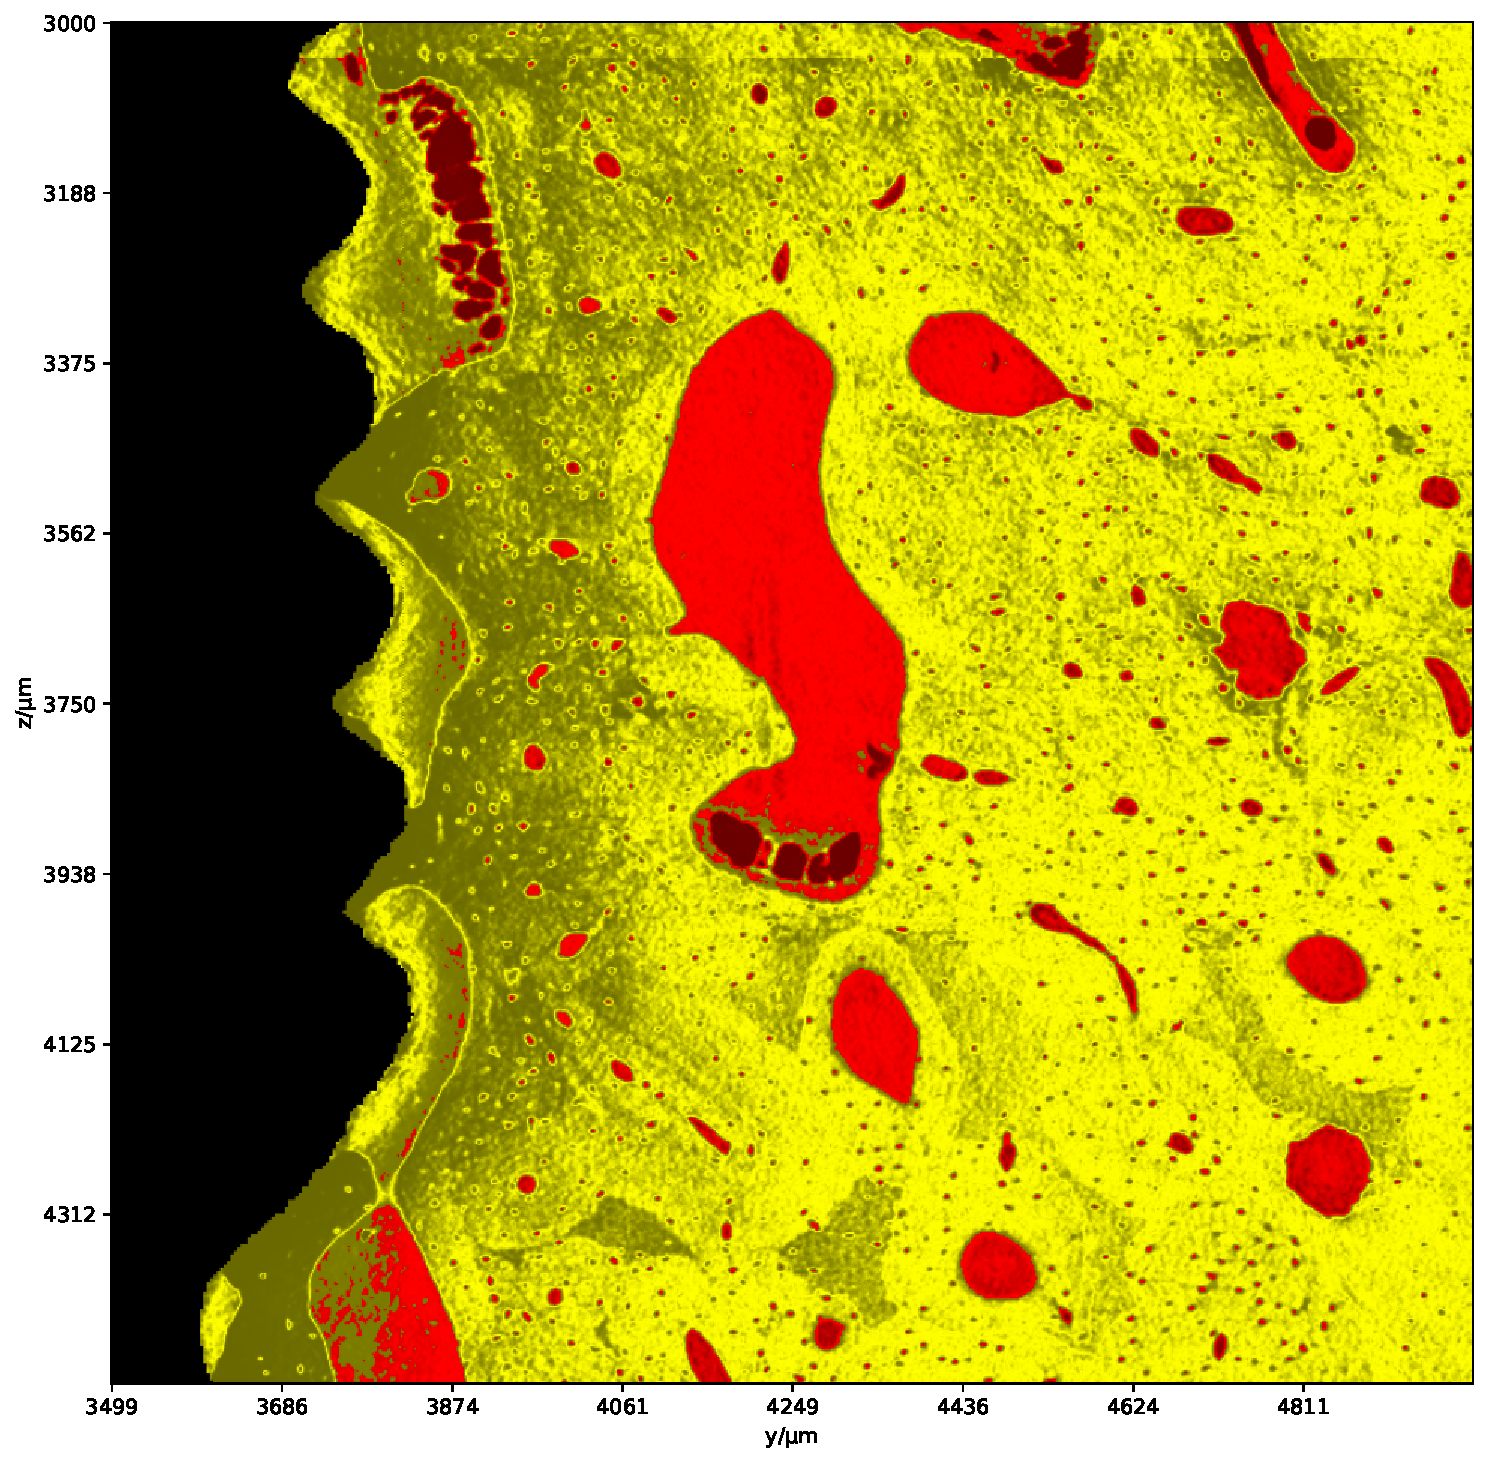
\includegraphics[width=.45\linewidth]{generated/770c_pag_global_zy.pdf} \\
    \end{tabular}
    \caption{
	YZ-slices of the original tomography (top left), Otsu segmentation (top
	right), our classification (bottom left), and global threshold
	classification (bottom right).  Yellow depicts bone and red depicts
	soft tissue. Note that our segmentation correctly classifies the
	materials close to the implant, and particularly in the grooves of the
	screw threads, whereas the global threshold and Otsu classification
	fails.
    }
    \label{fig:histology-comparison2}
\end{figure*}

We see that our segmentation is overall successful in identifying actual
features, rather than artifacts, and classifying the internal darker regions as
soft tissue and the lighter regions as bone. This is further confirmed in
\Cref{sec:blood-network}. However, extremely close to the implant (a few
voxels), we cannot verify the segmentation, as the voxel values are so blended
together with the implant voxel values that they become indistinguishable. A
further strengthening of the analysis is needed to reach this layer. It is
possible that the information is irretrievably lost, or perhaps it can be
retrieved through a different method, such as deconvolution.  It also fails
within some of the soft tissue blobs, which is due to air bubbles in the resin,
which have a very low density and therefore a very low absorption.

\subsection{Quantitative evaluation}

% Why it is a problem
Reliably evaluating segmentation methods on medical data such as that
presented in this paper is a challenging task. A satisfactory annotated ground
truth does not exist, which makes quantitatively evaluating one method against
another very hard. Furthermore, due to the very large number of voxels, using
manual or semi-automatic methods quickly becomes impractical. One such example
are neural networks, which need to be trained on multiple instances of similar
data accompanied by an annotated ground truth. This is a very time consuming
and expensive procedure, and does not easily translate to other data, which are
only slightly dissimilar.

% How are we going to approach it
To ensure a reliable and consistent verification of our method, we must tackle
a common problem: solutions are often hard to reproduce and thus
verify~\cite{replication-crisis}. We attempt to overcome this difficulty by
creating synthetic reproducible data, accompanied by a consistent reference
level ground truth. The generated data resembles our original data and shares
many physical qualities, but instead of being acquired at ESRF, it is simulated
using the software Novi-sim~\cite{novisim} on a consumer-grade workstation.
Using simulations allow other researchers to not only reproduce but also modify
our tomographic models and perform new experiments. This will both extend the
robustness of our segmentation, and make it less specific and dependent on our
original data.  In future experiments this also allows to extract 2D-slices of
synthetic data and compare with manually inspected and annotated histologies.

% TODO (Alle): placeret det forkerte sted måske? I hvert fald ikke helt optimalt.
% kan vi finde en bedre placering til dette?
Original data and synthetic data, with STL files and ground truth have been
made freely available \ref{sec:pubdata}.

\subsubsection{Ground truth and synthetic data}

% How we use Novi-sim
The presented segmentation pipeline results in a set of masks, one for each
material.  Each mask is overlayed unto a single volume representing our
artificially constructed ground truth. By construction, it will have a perfect
overlap, correctly identifying each material using our method.  The masks for
each material are converted into meshes and used to generate STL files.  The
generated STL files are transformed to synthetic tomograms using Novisim.
While the software is set up to simulate the original experiment at ESRF, it
will naturally not be a perfect match. The generated ground truth is now
perfectly accurate with the input, but deviates slightly but predictably from
the generated tomogram due to experimental physical effects and artifacts. This
allows us to use reproducible synthetic data to consistently compare our
segmentation method with other and detect in which regions they differ the
most. Because regions very close and very far away from the implant are
difficult, any intermediate regions should be fairly consistent across methods.
Finally we can inspect the differing regions visually to evaluate on the
overall performance. This results in a drastically reduced volume needed to be
manually inspected.

% TODO (Aleksandar): how did it go then?
% Discussion about the results and performance of the simulated data
% Summarize the findings using a table with error measures relative to ground truth
% So what we look at here is purely how accurate the segmentation is relative to gtruth,
% and not anything in regard to application, i.e. one BIC-score relative to another makes
% little sense to discuss here
% for example, L2, L1, "typically used ml-confidence scores" weighted by model confidence
% and other measures... see uploaded notes
\begin{table}[]
\caption{Score of methods using different error-measures.}
\label{tab:scores}
\centering
\begin{tabular}{lllll}
\toprule
Method           & M1 & M2 & M3 & M4 \\
\midrule
Ours             & -- & -- & -- & -- \\
Global threshold & -- & -- & -- & -- \\
Otsu             & -- & -- & -- & -- \\
\bottomrule
\end{tabular}
\end{table}

% TODO (James), omdøb nedenstående subsection til mere passende navn, egentlig
% er det jo mere motivation og application osv.
\subsection{Dataset analysis}

Having verified the method qualitatively and quantitatively, we can have a more
detailed look into the segmented data. We are interested in the blood vessel
network in the bone region and the tissue-to-implant contact. We will start by
analyzing the blood vessel network and then the tissue-to-implant contact.

\subsubsection{Blood vessel network}
\label{sec:blood-network}

With a good separation of soft tissue and bone, we map out the blood vessel
network using connected components analysis, which is visualized in the 3D
renders in~\Cref{fig:blood-network}. Here we see that we have successfully
segmented the blood vessels out of the bone region. It is especially prominent
when looking at the capillary network, as we can see these in fine detail.
Noteworthy, the newly formed bone region (\Cref{fig:blood-new-slice}) contains
larger concentrations of small blood vessels, compared to the old bone
(\Cref{fig:blood-old-slice}). If we zoom in on a small cube region
(\Cref{fig:blood-old-cube} and \Cref{fig:blood-new-cube}), we see it even more
defined, clearly seeing how the larger vessels connect through the smaller
ones.

\begin{figure}
    \centering
    \begin{subfigure}[b]{\linewidth}
    \centering
        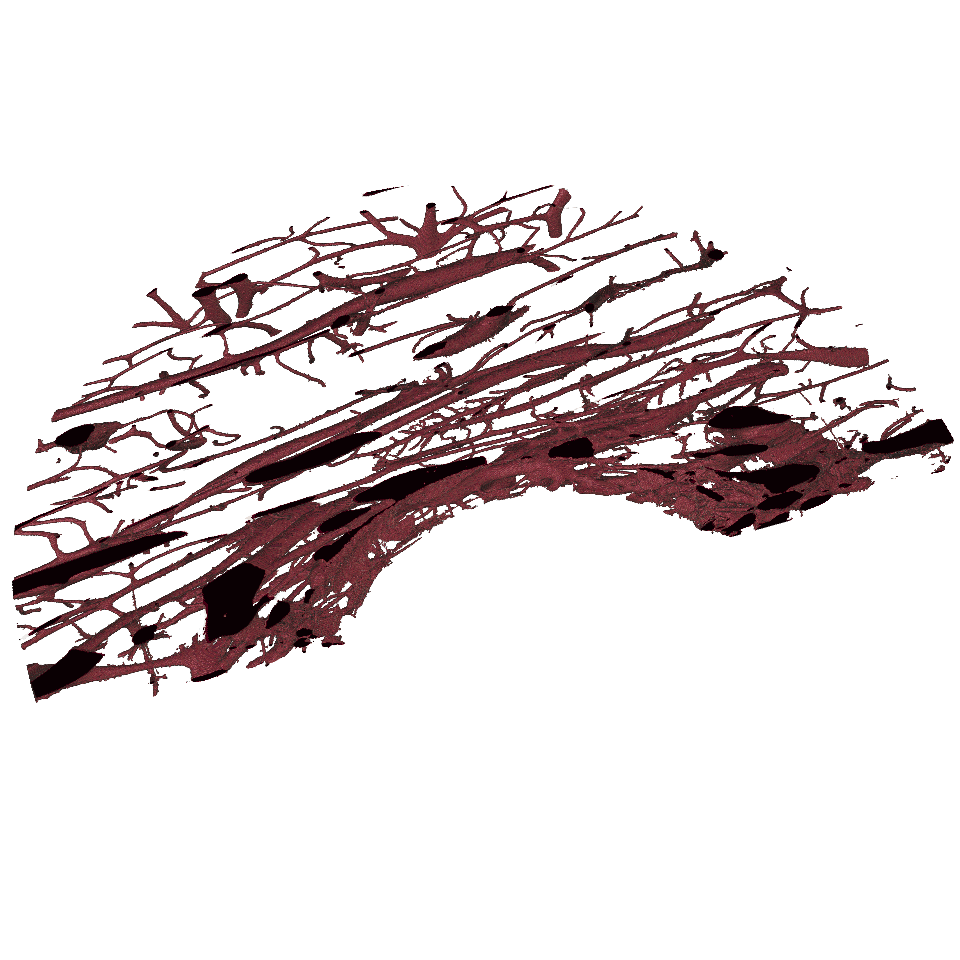
\includegraphics[width=.7\linewidth]{generated/figure10_old_bone.png}
	% TODO (Alle): opdater hvis en anden slice størrelse bliver brugt. voxel size = 3.75
        \caption{A 375 µm $\times$ 4230 µm $\times$ 6480 µm slice of the blood network in the old bone region.}
        \label{fig:blood-old-slice}
    \end{subfigure}
    \begin{subfigure}[b]{\linewidth}
    \centering
        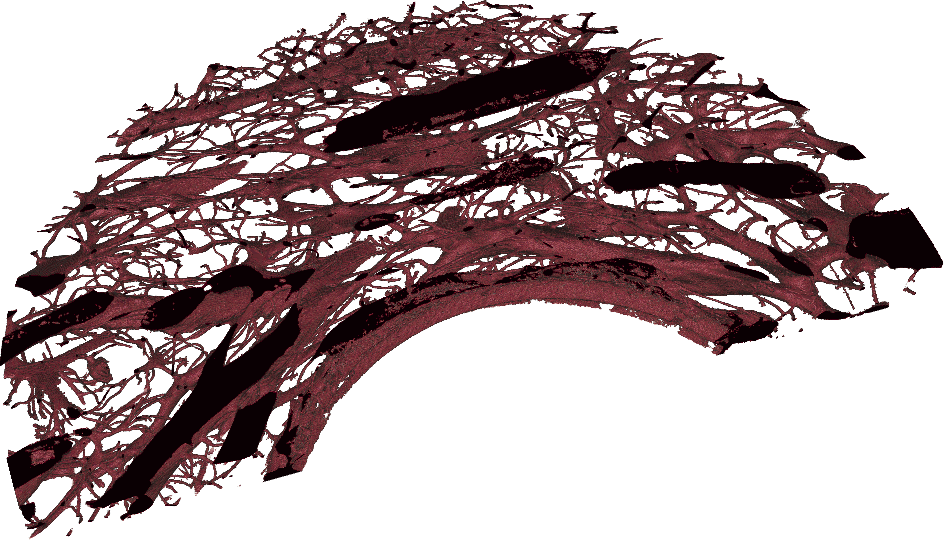
\includegraphics[width=.7\linewidth]{generated/figure10_new_bone.png}
        \caption{A 375 µm $\times$ 4230 µm $\times$ 6480 µm slice of the blood network in the new bone region.}
        \label{fig:blood-new-slice}
    \end{subfigure}
    \begin{subfigure}[b]{.48\linewidth}
    \centering
        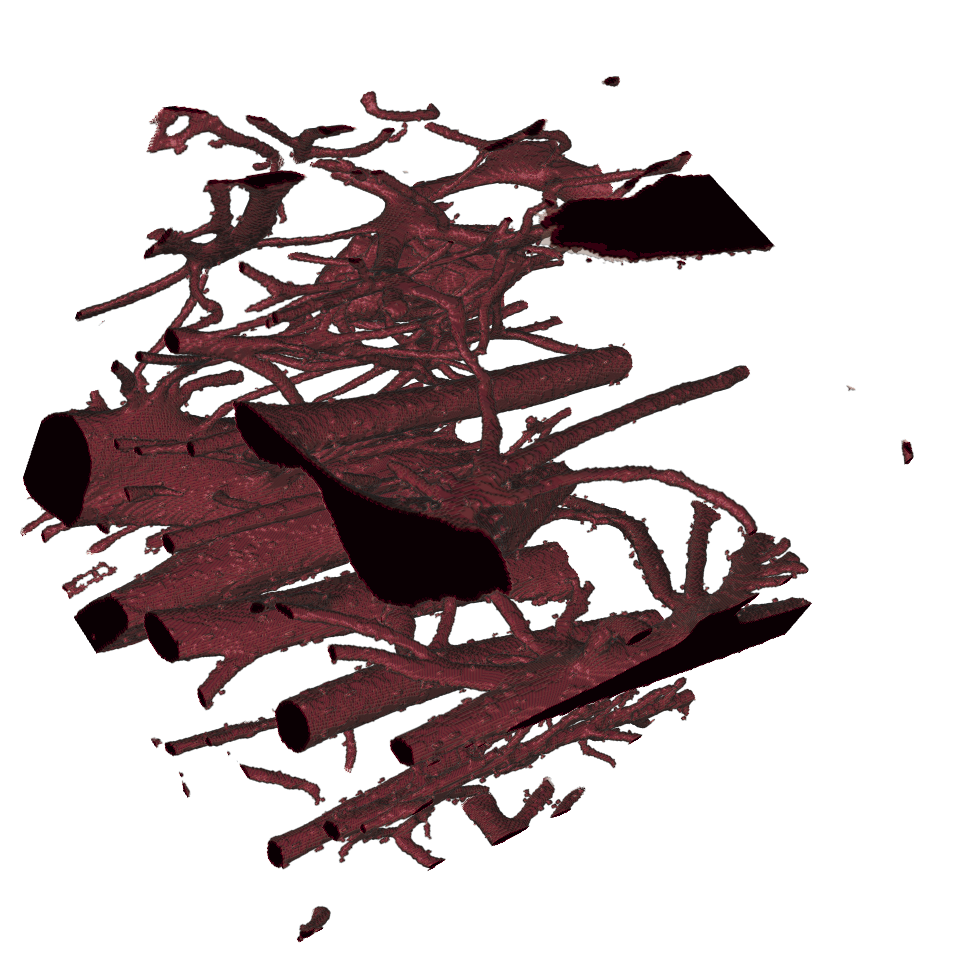
\includegraphics[width=.9\linewidth,height=\linewidth]{generated/figure10_old_cube.png}
        \caption{A $1mm \times 1 mm \times 1 mm$ cube of the blood network in the old bone region.}
        \label{fig:blood-old-cube}
    \end{subfigure}
    \hfill
    \begin{subfigure}[b]{.48\linewidth}
    \centering
        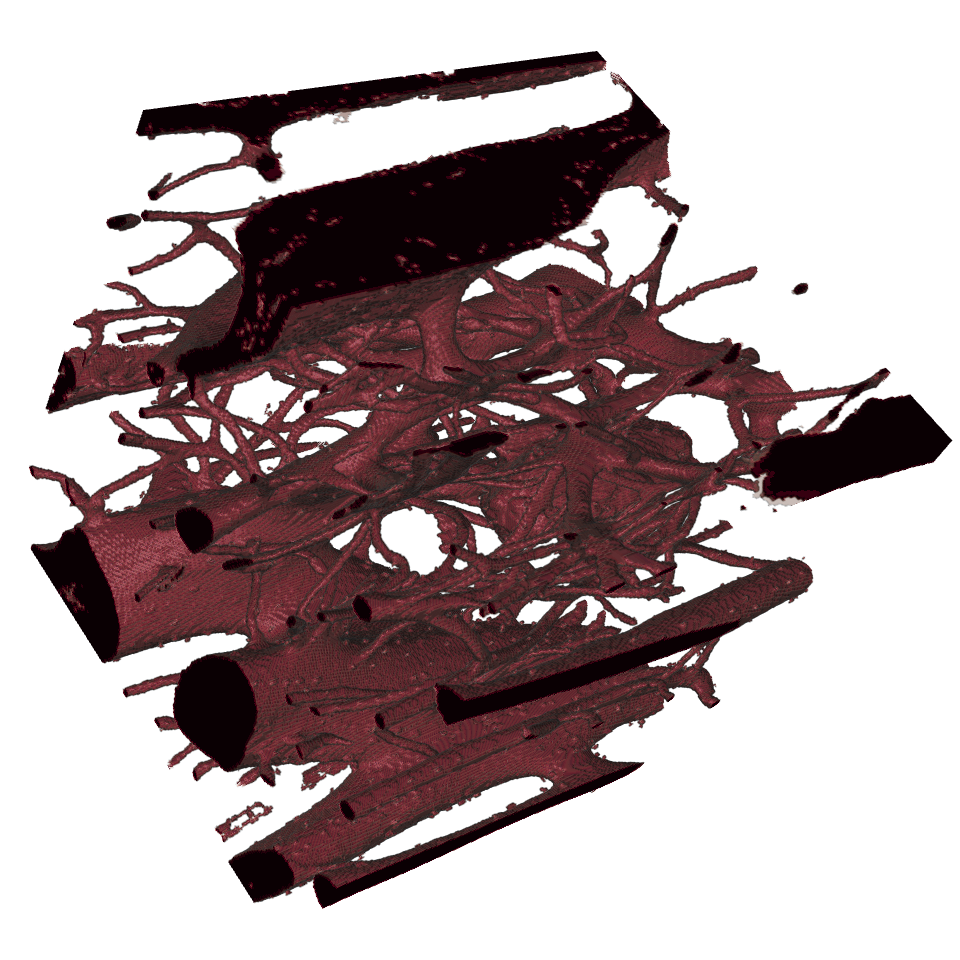
\includegraphics[width=.9\linewidth,height=\linewidth]{generated/figure10_new_cube.png}
        \caption{A $1mm \times 1 mm \times 1 mm$ cube of the blood network in the new bone region.}
        \label{fig:blood-new-cube}
    \end{subfigure}
    \caption{
        3D renders of the blood network. We see a difference between the
        capillary network in the old bone region
        (\ref{fig:blood-old-slice},\ref{fig:blood-old-cube}) compared to the
        newly grown bone region
        (\ref{fig:blood-new-slice},\ref{fig:blood-new-cube}), where the new
        bone region contains a higher concentration of small blood vessels,
        compared to the old bone region containing fewer larger blood vessels.
    }
    \label{fig:blood-network}
\end{figure}

\subsubsection{Implant contact}
\label{sec:contact}

Tissue in contact with the implant can be studied using the EDT from the
implant, restricted to the bone region. We can simply mask the voxels that are
within a thin shell of distances, $d_{min} < d(x,y,z) \le d_{max}$, for
example, $d_{min} = 1 \text{µm}$ to $d_{max} = 5 \text{µm}$. We then sum over
the masked voxels of each tissue type to obtain and divide by the total to
obtain the tissue-to-implant contact per area or study the distribution across
the surface area qualitatively. In particular, we are interested in the
difference between the old and new bone regions. We define the metric as
follows:

\begin{equation}
    BIC = \frac{\sum_{i : \text{field}(i) < 5} \text{bone}(i)}{\sum_{i : \text{field}(i) < 5} \text{voxels}(i)}
\end{equation}

We find the old and new bone regions at different $z$ levels, based on the
threading of the implant, with new bone being near the small threads and old
bone being near the large threads. The results can be seen in \Cref{tab:bic}.
We see that the BIC is higher in the old bone region than in the new bone
region, which is expected as the bone grows around the implant over time. This
is further confirmed by the blood vessel network analysis, as the new bone
region contains a higher concentration of small blood vessels, indicating that
the bone is still growing. This shows that the method is successful in
segmenting the bone and soft tissue regions and that the segmentation can be
used to study BIC.

\begin{table}
    \caption{The mean and standard deviation of bone-to-implant contact in the old and new bone regions for each of our samples.}
    \label{tab:bic}
    \centering
    \begin{tabular}{lcc}
        \toprule
        Sample & Old bone & New bone \\
        \midrule
        770\_pag & $0.5020 \pm 0.1222$ & - \\
        770c\_pag & $0.6519 \pm 0.1055$ & $0.5638 \pm 0.0907$ \\
        771c\_pag & $0.4517 \pm 0.1708$ & $0.5016 \pm 0.1078$ \\
        772\_pag & $0.7012 \pm 0.1065$ & $0.5222 \pm 0.0869$ \\
        775c\_pag & $0.2802 \pm 0.0928$ & $0.2652 \pm 0.1054$ \\
        810c\_pag & $0.6819 \pm 0.0866$ & $0.5155 \pm 0.0897$ \\
        811\_pag & $0.5832 \pm 0.1015$ & $0.3715 \pm 0.0935$ \\
        \bottomrule
    \end{tabular}
\end{table}

